%%
%
% ARQUIVO: cap-01.tex
%
% VERSÃO: 1.0
% DATA: Maio de 2016
% AUTOR: Coordenação de Trabalhos Especiais SE/8
% 
%  Arquivo tex de exemplo de capítulo do documento de Projeto de Fim de Curso.
%
% ---
% DETALHES
%  a. todo capítulo deve começar com \chapter{•}
%  b. usar comando \noindent logo após \chapter{•}
%  c. citações para referências podem ser
%       i. \citet{•} para citações diretas (p. ex. 'Segundo Autor (2015)...'
%       ii. \citep{•} para citações indiretas (p. ex. '... (AUTOR, 2015)...'
%  d. notas de rodapé devem usar dois comandos
%       i. \footnotemark para indicar a marca da nota no texto
%       ii. \footnotetext{•}, na sequência, para indicar o texto da nota de rodapé
%  e. figuras devem seguir o exemplo
%       i. devem ficar no diretório /img e devem ser no formato EPS
%  f. tabelas devem seguir o exemplo
%  g. figuras e tabelas podem ser colocadas em orientação landscape
%       i. figuras: usar \begin{sidewaysfigure} ... \end{sidewaysfigure}
%                   em vez de \begin{figure} ... \end{figure}
%       ii. tabelas: usar \begin{sidewaystable} ... \end{sidewaystable}
%                    em vez de \begin{table} ... \end{table}
%  h. toda figura e tabela deve ser referenciada ao longo do texto com \ref{•}
% ---
%%

\chapter{Introdução}
\noindent
O objetivo deste trabalho é desenvolver um algoritmo que classifique uma questão inédita de concurso dentre um conjunto de assuntos pré-determinados. Para atingir este objetivo, serão exploradas técnicas de aprendizado de máquina e processamento de linguagem natural.


\section{Motivação}
%porque estudar o tema é importante/relevante?

\subsection{Plataformas de auxílio ao aprendizado}
Neste relatório, será entendido por PAA qualquer software que tenha objetivo pedagógico. Existe um mercado de educação à distância (EAD) que por seu caráter remoto, propicia o uso de tecnologia digital para a facilitação do ensino.  Esse mercado tem se tornado competitivo e ganhado cada vez mais importância.

\subsection{Classificação automática de assuntos}

Será entendido por CAA qualquer método de classificação de textos exequível via software sem auxílio de um operador. Os principais métodos existentes são listados na seção de Métodos.
A CAA já é amplamente utilizada na indústria, por exemplo, em sites de notícias, gerenciadores de emails ou motores de busca.

\subsection{Loona}
Loona é um motor de busca em desenvolvimento pela empresa PaperX. Trata-se de uma ferramenta de busca de vídeos por imagem.

\begin{figure}[!ht]
	\centering
	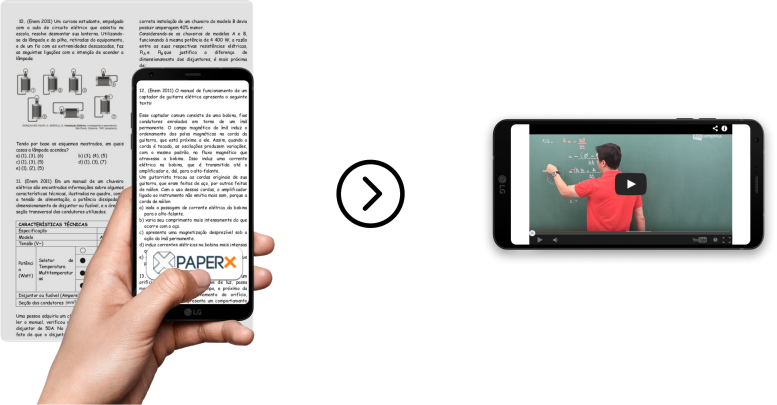
\includegraphics[width=0.4\textwidth]{figures/loona.png}   
	\caption{Funcionamento do loona}
	\label{fig:loona}
\end{figure}


\section{Objetivo}
%que tentará ser alcançado (principal e secundários)
O funcionamento do motor de busca em questão é dividido em três etapas:
\begin{itemize}
\item Reconhecimento ótico de caracteres (OCR); 
\item Classificação de texto e
\item Busca
\end{itemize}

\begin{figure}[!ht]
	\centering
	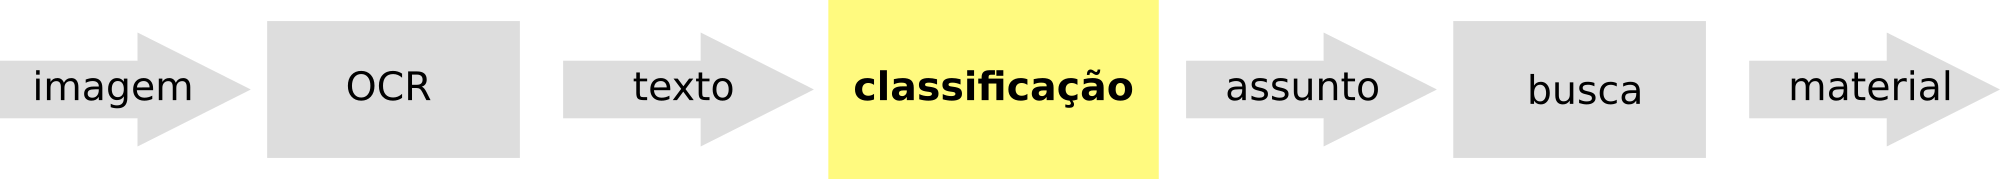
\includegraphics[width=0.4\textwidth]{figures/fluxograma.png}   
	\caption{Fluxo funcional da ferramenta}
	\label{fig:fluxograma}
\end{figure}


Este trabalho será restrito a etapa central: Classificação de texto.


% \section{Justificativa}
%a importância do trabalho no contexto institucional

\section{Metodologia}
%como o trabalho deverá ser conduzido
A primeira etapa do trabalho corresponde à obtenção de dados para serem utilizados nos algoritmos de aprendizado de máquina. Isso é feito a partir de Web scraping de questões de concursos públicos já rótuladas com os seus respectivos assuntos.

Em seguida, há uma fase de processamento de dados que remove inconsistências e prepara uma interface ideal para os algoritmos que serão aplicados posteriormente.

A terceira fase é a parte central do trabalho e consiste em explorar diferentes modelos para a classificação de questões. Cada um desses modelos possui suas particularidades com diferentes arquiteturas e hiperparâmetros para uma otimização de acordo com o contexto dos dados utilizados.

Como etapa final, a solução ótima encontrada de classificação é implementada na plataforma de auxílio ao aprendizado da paperx.com.br para o uso em ferramentas de busca.


\section{Estrutura}
%do documento
Sobre os capítulos subsequentes a seguinte distribuição de conteúdo:
\begin{itemize}
\item Capítulo 2: 
fundamentação teórica sobre cada um dos algoritmos de classificação que serão utilizados;
\item Capítulo 3:
descrição da implementação para cada uma das etapas descritas na metodologia;
\item Capítulo 4:
comparação dos resultados dos entre diferentes modelos implementados.
\end{itemize}